\section{Operational Semantics}

\begin{figure*}[!t]
\raggedright
%
\textbf{Syntax}\\
%
\begin{smathpar}
\renewcommand{\arraystretch}{1.2}
\begin{array}{lclcl}
\multicolumn{5}{c} {
  t \in \mathtt{Thread\; Ids} \qquad
  x,y \in \mathtt{Variables} \qquad
  c \in \mathtt{\{()\}} \cup \mathbb{N} \qquad
}\\
v & \in & \mathtt{Values} & \coloneqq & c \ALT \lambda x.\,s\\
s & \in & \mathtt{Expressions} & \coloneqq & v \ALT s\;s \ALT \run{s}{s}
   \ALT \fork{s} \ALT \pull \ALT \push{s}\\
p & \in & \mathtt{Programs} & \coloneqq & s_t \ALT p\,||\,p \\
f & \in & \mathtt{Tags} & \coloneqq & \C{INIT} \ALT \C{FORK} \;b 
  \ALT \C{PUSH} \ALT \C{MERGE} \;b\\
b & \in & \mathtt{Branches} & \coloneqq & [(v,f)] \ALT (v,f)::b \\
\end{array}
\end{smathpar}
%
\bigskip
%% If we are feeling adventurous, we can try defining e and s 
%% mutually recursively, such that their evaluation relations 
%% are also mutually recursive (multiple reduction steps of one 
%% relation is a single step of other). 

%
\textbf{Evaluation Contexts}\\
%
\begin{smathpar}
\renewcommand{\arraystretch}{1.2}
\begin{array}{lclcl}
H & \in & \mathtt{Branch\; Histories} & \coloneqq & t \mapsto b\\
E & \in & \mathtt{Eval.\; Contexts}(s) & \coloneqq & \bullet \ALT 
  \bullet\;s \ALT v\;\bullet \ALT \run{\bullet}{s}\\
P & \in & \mathtt{Eval.\; Contexts}(p) & \coloneqq & E_t \ALT 
  \bullet\,||\,p \ALT p\,||\,\bullet \\
\end{array}
\end{smathpar}
%
\bigskip

%
\textbf{Reduction Relation} \quad \fbox {$p;\;H \stepsto p';\;H'$} \\
%
%
\begin{smathpar}
\begin{array}{lcll}
(\run{v}{s})_t;\cdot & \stepsto & 
  s_t; \cdot[t_{\top} \mapsto [(v,\C{INIT})]]
            [t\mapsto [(v,\C{FORK}\; [(v,\C{INIT})])]] 
            & [\rulelabel{E-Run}]\\
(\fork{s})_t;H(t\mapsto (v,\_)::b) & \stepsto & 
    ()_t\,||\, s_{t'}; H[t'\mapsto [(v, \C{FORK} H(t))]] 
    \spc \texttt{where}\; t'\not\in dom(H)
            & [\rulelabel{E-Fork}]\\
(\push{v})_t;H & \stepsto & ()_t;H[t \mapsto (v,\C{PUSH})::H(t)]
            & [\rulelabel{E-Push}]\\
% & & & v\,=\,\C{merge}\,v\,v_1\,v_2 ~\texttt{and}~ \\
((\lambda x.s)\;v)_t;H & \stepsto & ([v/x]\,s)_t;H
            & [\rulelabel{E-App}]\\
(\pull)_t;H(t \mapsto (v,\_)::m) & \stepsto & v_t;H
            & [\rulelabel{E-Pull}]\\
\end{array}
\end{smathpar}
%

% %
% \hspace*{\fill}[\rulelabel{E-Admin}]\hspace*{0.25in}
% \begin{smathpar}
% \begin{array}{c}
% \RULE
% {
%   s_t; H ~\stepsto^{*}~ v_t; H
% }
% {
%   E_t[s]; H ~\stepsto^{*}~ E_t[v]; H
% }
% \end{array}
% \end{smathpar}
% %

%
\hspace*{\fill}[\rulelabel{E-Pull-Wait}]
\begin{smathpar}
\begin{array}{c}
\RULE
{
  t\neq t' \spc
  \under{H}{v' \mbleto v} \spc
% \C{world}(H,t') \semsucceq \C{world}(H,t)\spc 
  v_m = \C{merge}(\C{lca}(H(t),H(t')), v, v') \spc
}
{
  (\pull)_t;H(t \mapsto (v,f)::m)(t' \mapsto (v',\_)::\_) ~\stepsto~
  (\pull)_t;H[t \mapsto (v_m,\C{MERGE}\; H(t'))::(v,f)::m]
}
\end{array}
\end{smathpar}
%

\caption{\name: Syntax and Operational Semantics}
\label{fig:opsem}
\end{figure*}


We formalize our ideas in the context of a lambda calculus ($\lang$)
shown in Fig.~\ref{fig:opsem}. Expressions of $\lang$ are variables,
constants, and \name primitives composed using the lambda combinator.
For brevity, we use short names for \name primitives: \C{run} for
\C{with\_init\_version\_do}, and \C{fork} for \C{fork\_version}. To
simplify the technical development, \name's \C{sync\_next\_version}
operation is broken down into two primitives - \C{push} and \C{pull},
which can be lambda-composed get the desired effect:
\begin{smathpar}
  \C{sync}\;x \;=\; (\lambda y.\pull)\; (\push\,x)
\end{smathpar}
The semantics of\C{get\_current\_version} is subsumed by \C{pull},
hence elided.  Values ($v$) are constants and lambda abstractions.  A
program ($p$) is a parallel composition of threads, where each thread
is an expression ($s$) indexed by the corresponding thread identifier
($t$). 

Fig.~\ref{fig:opsem} also shows the syntax of \emph{branches}, which
are the artifacts of evaluation and only appear during the run-time. A
branch is a non-empty sequence of tagged values, where the tag
captures the abstract run-time operation that led to the creation of
the value. It is implicitly assumed that each value added to a branch
is uniquely identifiably, hence no two values on a branch are equal.
The uniqueness assumption is later extended to a collection of
branches that constitute a branching structure. A real implementation
meets this assumption by versioning values across the branches. Thus,
in reality, branches contain \emph{versions} which denote values. The
semantics, however, doesn't make this distinction, and uses values and
versions interchangeably.

Small-step operational semantics of $\lang$ is defined via reduction
relation ($\stepsto$) that relates \emph{program states}. A program
state ($p;\,H$) consists of a program $p$ and a \emph{branch history}
$H$ that maps thread Ids to corresponding branches; each thread is
associated with a branch during the evaluation. Evaluation contexts
have been defined separately for expressions ($E$) and programs ($P$),
with the latter subsuming the former. $E$ is defined to evaluate the
first argument of a \C{run} expression to a value that constitutes the
initial version (recall that \C{run} models \name's
\C{with\_init\_version\_do}). Program evaluation context
non-deterministically picks one of the threads to evaluate. The admin
rule that relates transitions of holes to transitions of expressions
and programs is straightforward, hence elided. Rest of the reduction
rules are presented in Fig.~\ref{fig:opsem}. For brevity, we write
$H(t\mapsto (v,f))$ to denote the proposition that $H$ maps $t$ to
$(v,f)$. The notation $H[t \mapsto (v,f)]$ as usual denotes
the extension of $H$ with the binding $t \mapsto (v,f)$.

Reduction rules let expression evaluation take a step by rewriting the
expression and suitably updating the branch history ($H$). The
\rulelabel{E-Run} rule is applicable only when $H$ is empty, i.e.,
when no prior branching structure exists. The rule rewrites the
$\C{run}\;v\;s$ expression to $s$, while creating a new branching
structure with two branches: a \emph{top} branch that has just the
initial version (tagged with \C{INIT}), and a branch for the current
thread ($t$) forked-off from the top branch.  The first version on the
current branch ($H(t)$) denotes the same value ($v$) as the initial
version on the top branch, although versions themselves are deemed
distinct. The new version is tagged with a \C{FORK} tag that keeps the
record of its orgin, namely the \C{fork} operation and the branch from
which the current branch is forked. The \rulelabel{E-Fork} rule forks
a new thread with a fresh id ($t'$) and adds it to the thread pool.
The corresponding branch ($H(t')$) is forked from the parent thread's
branch ($H(t)$). The semantics of branch forking is same as described
above. The \C{fork} expression in the parent thread evaluates to
\C{()}. The \rulelabel{E-Push} rule creates a new version on the
current branch ($H(t)$) using the pushed value ($v$).
\rulelabel{E-App} is the standard beta reduction rule.

The semantics non-deterministically chooses \rulelabel{E-Pull} or
\rulelabel{E-Pull-Wait} rules to reduce a \C{pull} expression. The
\rulelabel{E-Pull} rule reduces \C{pull} to \C{()}, and returns the
latest version on the current branch. The \rulelabel{E-Pull-Wait} rule
can be thought of as a stutter step; it doesn't reduce \C{pull}, but
updates the branching structure by merging (the latest version of) a
concurrent branch ($H(t')$) into (the latest version of) the current
branch ($H(t)$), and extending the current branch with the merged
version ($v_m$). The new version is tagged with a \C{MERGE} tag that,
like a \C{FORK} tag, records its origin. The premises of the
\rulelabel{E-Pull-Wait} serve the important purpose of contraining the
branching structure by allowing only the legal merges, and
consequently preserving certain desirable properties of the system;
we will go into the details shortly. The \rulelabel{E-Pull-Wait} and
\rulelabel{E-Pull} rules thus let a thread sync with a subset of
concurrent threads in multiple steps before returning the result of
the \C{pull}. Since \C{sync} is a composition of \C{push} and
\C{pull}, its behavior can be explained thus: \C{sync} pushes the
given value onto the current (local) branch, merges a (possibly empty)
subset of concurrent branches into the local branch, and returns the
result.

We will not present a series of definitions and results that let us
understand the premises of the \rulelabel{E-Pull-Wait} rule, examine
the merge operation in closer detail, and appreciate the need for
constraining the branching structure. First, we formalize the
intuitive notation of the ancestor relationship between versions of a
legal branching history (i.e., a branching history generated by the
rules in Fig.~\ref{fig:opsem}):

\begin{definition} [\bfseries Ancestor]
Version $v_1$ is a ancestor of version $v_2$ under a history
$H$ (written $\under{H}{v_1 \preceq v_2}$) if and only if one of the
following is true:
\begin{itemize}
  \item There exists a branch $b$ in $H$ (i.e., $\exists(t\in
  dom(H)).\,H(t) = b$) in which $v_2$ immediately succeeds
  $v_1$,
  \item There exists a branch $b$ in $H$ that contains $(v_2, 
  \C{FORK}\; (v_1,f_1)::b_1)$, for some $f_1$ and $b_1$,
  \item There exists a branch $b$ in $H$ that contains
  $(v_2, \C{MERGE}\;(v_1,f_1)::b_1)$, for some $f_1$ and $b_1$,
  \item $v_1 = v_2$, or $v_1$ is transitively a ancestor of
  $v_2$, i.e., $\exists v.~ \under{H}{v_1 \preceq v} \conj
  \under{H}{v \preceq v}$ 
\end{itemize}
\end{definition}

Ancestor relation is therefore a partial order (reflexive, transitive,
anti-symmetric) with a greatest lower bound (the initial version).
Thus, for any two versions in a legal history, there exist at least
one common ancestor. Ancestor relationships among the common ancestors
let us define the notion of a least common ancestor (LCA):

\begin{definition} [\bfseries Least Common Ancestor]
Version $v$ is said to be a common ancestor of versions $v_1$ and
$v_2$ under a history $H$ if and only if $\under{H}{v \preceq v_1}$
and $\under{H}{v \preceq v_2}$. It is said to be the least common
ancestor (LCA) of $v_1$ and $v_2$, iff there does not exist a $v'$
such that $\under{H}{v' \preceq v_1}$ and $\under{H}{v' \preceq v_2}$
and $\under{H}{v \preceq v'}$.
\end{definition}

\begin{figure}
\centering
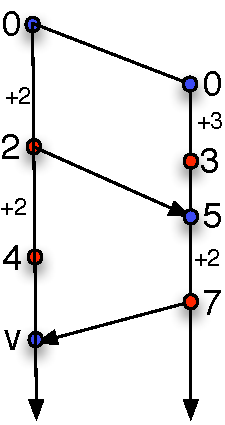
\includegraphics[scale=0.6]{Figures/merge-needs-lca}

\caption{This example of a grow-only counter illustrate why \C{merge}
needs a least common ancestor, and not just a common ancestor. Both 0
and 2 are common ancestors of 4 and 7, while 2 is their least common
ancestor (since $0 \preceq 2$). The result (v) of merging 4 and 7 is
11 (incorrect) if 0 is used as the common ancestor for merge, and 9
(correct, because 2+2+3+2 = 9) if 2 is used. }
\label{fig:merge-needs-lca}
\end{figure}

\begin{figure}[!t]
\centering
\subcaptionbox[] {\small
  In this example, 1 and 3 have two LCAs (3 and 4) a result of
  previous merges. The dotted circle denotes a virtual ancestor
  obtained by merging the two LCAs.
  \label{fig:criss-cross-lcas}
} [0.47\columnwidth] {
  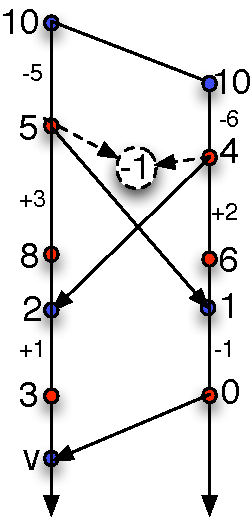
\includegraphics[scale=0.55]{Figures/2-LCAs}
}
\hfill
\subcaptionbox[] {\small
  In this example, 3 and 6 have two LCAs (2 and 1) despite there not
  being any previous merges between their respective branches.
  \label{fig:external-lcas}
} [0.47\columnwidth] {
  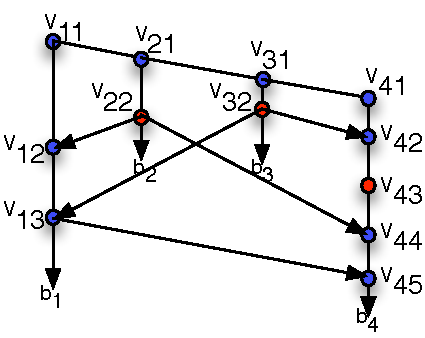
\includegraphics[scale=0.7]{Figures/2-external-LCAs}
}
\caption{Examples where merging versions have more than one LCA}
\label{fig:many-lcas}
\end{figure}

When merging two concurrent versions $v_1$ and $v_2$, the common
ancestor argument for \C{merge} must the LCA of $v_1$ and $v_2$,
without which \C{merge} may yeild unexpected results. This is
demonstrated for the grow-only counter in
Fig.~\ref{fig:merge-needs-lca}, where incorrect count is obtained if a
common ancestor that is not an LCA is used to merge 4 and 7. While in
this example there is a unique LCA for 4 and 7, in general this may
not be the case. With unrestrained branching and merging, there is no
bound on the number of LCAs a pair of versions can have.
For example, in
Fig.~\ref{fig:criss-cross-lcas}, the merge of 1 with 3 is preceded by
two ``criss-cross'' merges between their respective branches resulting
in there being two LCAs (3 and 4) for 1 and 3. Multiple LCAs can
occur even without criss-cross merges, as demonstrated by
Fig.~\ref{fig:external-lcas}. 

\begin{definition} [\bfseries Internal and External Ancestors]
Given a branch $b$ and a version $v\in b$, an internal ancestor of $v$
is an ancestor from the same branch $b$. An external ancestor of $v$
is an ancestor from a different branch $b'\neq b$. 
\end{definition}

\begin{definition} [\bfseries Least Internal and External Ancestors]
Given a branch $b$ and a version $v\in b$, least internal ancestor is
the immediate ancestor version ($v_i$) of $v$ on $b$. Least external
ancestor ($v_o$) is an external ancestor of $v$ that is not an
ancestor of any other external ancestor of $v$. That is,
$\under{H}{v_o \preceq v}$, and there does not exist a $v_o' \not\in
b$ such that $\under{H}{v_o' \preceq v}$ and $\under{H}{v_o \preceq
v_o'}$. 
% We lift the definition to the level of branches; $v_o$ is an
% external locus of a branch $b$ iff it is an external locus of its
% latest version.
\end{definition}

Note that all branches (except $H(t_{\top})$) begin with a \C{FORK}
tag, hence every version has at least one least external ancestor. We
later prove that in the histories generated by the rules in
Fig.~\ref{fig:opsem}, the external ancestors of every version are
totally ordered, hence there is exactly one least external ancestor
for each version. We call the unique least external ancestor of a
version as its \emph{external locus}. Least internal ancestor, by
definition, is unique, which we sometimes call \emph{internal locus}.

\begin{definition} [\bfseries Mergeability]
Given a history $H$, a version $v_1$ and a version $v_2$ that is not
an ancestor of $v_1$ under $H$, $v_2$ is mergeable into $v_1$ (denoted
$\under{H}{v_2 \mbleto v_1}$) iff $v_1$'s external locus is an
ancestor of $v_2$, or $v_2$'s external locus is an ancestor of $v_1$.
\end{definition}

\begin{lemma} [\bfseries Unique External Locus]
Every version $v$ (except the \C{INIT} version) in the history $H$
generated by the rules in Fig.~\ref{fig:opsem} has a unique external
locus.
\end{lemma}
\begin{proof}
By case analysis on the reduction relation. In each case, we assume
that the unique external locus property holds for the initial history,
and prove that it holds for the final history.

In \rulelabel{E-Run} case, initial version is the unique external locus of
the new version on the new branch $H(t)$. In \rulelabel{E-Fork} case,
which creates the branch $H(t')$ by forking from $H(t)$, the latest
version on $H(t)$ is the external locus of the first version on
$H(t)$. In \rulelabel{E-Push} case, the version on $H(t)$ has the same
external locus as the previous latest version, which, premise says, is
unique. No new version is created in \rulelabel{E-Pull}. In
\rulelabel{E-Pull-Wait}, new version is created by merging the latest
version ($v'$) on $H(t')$ into the latest version $v$ on $H(t)$.
Premise says that $v$ has a unique external locus (call it $v_o$). The
new version $v_m$ inherits $v_o$ as a least external ancestor, and
also has $v'$ as another least external ancestor. However, since
$\under{H}{v' \mbleto v}$, we have $\under{H}{v_o \preceq v'}$, we
have $v'$ as the the external locus.
\qed
\end{proof}

%% If we are allowed to merge earlier versions on branches, then we
%% have a possibility of utmost two LCAs.

\begin{theorem} [\bfseries Unique LCA]
Every pair of versions $v_1$ and $v_2$ in the history $H$ generated by
the rules in Fig.~\ref{fig:opsem} have a unique least
common ancestor. 
\end{theorem}
\begin{proof}
By case analysis on the step relation. In each case, we assume that
the unique LCA property holds for the initial history, and prove that
it holds for the final history.

The \rulelabel{E-Run} case is trivial. The \rulelabel{E-Push} case
creates a new version ($v$) with \C{PUSH} tag at the end of a branch.
Let $v_1$ be the previous version on the branch, and let $v_2$ be any
other version. The premise is that $v_1$ and $v_2$ have a unique LCA
$v_0$. Observe that $v$'s internal locus is $v_1$ and its external
locus is same as that of $v_1$. Hence, all ancestors of $v_1$
(including itself) are also ancestors of $v$. Moreover, $v$ has no new
ancestors except itself, which is the latest version being added.
Hence, any common ancestor of $v_1$ and $v_2$ is also a common
ancestor of $v$ and $v_2$, while there cannot be new common ancestors.
Hence LCA of $v$ and $v_2$ is unique. The reasoning for
\rulelabel{E-Fork} is similar. The \rulelabel{E-Pull} case is trivial. 

The \rulelabel{E-Pull-Wait} case is where the merge happens. Version
$v'$ is merging into version $v$ to produce the next version $v_m$.
Let $v''$ be any version. From the premise, we know that $v$ and $v''$
have a unique LCA (call it $v_1$), and $v'$ and $v''$ have a unique
LCA (call it $v_2$). Also, we know that $v''$ has a unique external
locus (call it $v_3$). We now consider cases
\begin{itemize}
  \item $v_1$ and $v_2$ are external to both $v$ and $v'$: Hence $v_1$
  is an external ancestor of $v$, and $v_2$ is an external ancestor
  of $v'$. Since $v$ and $v'$ are mergeable, there must exist a $v_4$
  such that $\under{H}{v_1 \preceq v_4}$ and $\under{H}{v_1 \preceq
  v_4}$, and either $\under{H}{v_4 \preceq v}$ or $\under{H}{v_4
  \preceq v'}$.  are external ancestors of
  $v_2$. Hence,
  $\under{H}{v_0 \preceq v_3} \conj \under{H}{v_1 \preceq v_3}$.
  Since $\under{H}{v_0 \preceq v_m} \conj \under{H}{v_1 \preceq v_m}$, 
  $v_2$ and $v_m$ have a unique LCA.

  \item $v_0$ is an internal ancestor of $v_2$, hence an external
  ancestor of $v$, hence an external ancestor of $v_m$. $v_1$ is
  an ancestor of $v'$, hence also an external ancestor of $v_m$. 
\end{itemize}


As proved
before, the merged version ($v_m$) has a unique external locus, which
is the merging version ($v'$).
\end{proof}

